\documentclass[a4paper, 11pt]{article}

\usepackage[utf8]{inputenc}
\usepackage{a4wide}
\usepackage{relsize}
\usepackage{graphicx}
\usepackage{float}
\usepackage[pdfborder={0 0 0}]{hyperref}
\usepackage{cleveref}
\usepackage{minted}
\usepackage{indentfirst}
\usepackage{setspace}

\onehalfspacing

\title{Big Data \& Cloud Computing \\ [0.8em] \smaller Pipelines \& Dataflows}
\author{Rui Fernandes}
\date{April 2022}

\AtBeginEnvironment{minted}{\let\itshape\relax}

\begin{document}

\maketitle

\section{Apache Beam}

\begin{minted}{py}
start_time = time.time()

with beam.Pipeline() as pipeline:
    lines = (
        pipeline
        | 'Read lines from text file' >> beam.io.ReadFromText(args.input_file)
        | 'Extract words' >> beam.FlatMap(lambda x: re.findall(r'[A-Za-z\']+', x))
        | beam.combiners.Count.PerElement()
        | beam.MapTuple(lambda word, count: '%s: %s' % (word, count))
        | 'Write to output file' >> beam.io.WriteToText(args.output_path)
    )

elapsed_time = time.time() - start_time
print('Elapsed time: {:.3f} seconds'.format(elapsed_time))
\end{minted}

\section{PySpark}

\begin{minted}{py}
start_time = time.time()

# create Spark context with necessary configuration
sc = SparkContext('local', 'PySpark Word Count Exmaple')

# read data from text file and split each line into words
words = sc.textFile(args.input_file).flatMap(lambda line: line.split(' '))

# count the occurrence of each word
wordCounts = words.map(lambda word: (word, 1)).reduceByKey(lambda a, b: a + b)

# save the counts to output
wordCounts.saveAsTextFile(args.output_path)

elapsed_time = time.time() - start_time
print('Elapsed time: {:.3f} seconds'.format(elapsed_time))
\end{minted}

\vspace{\baselineskip}

\section{Sequential}

\begin{minted}{py}
start_time = time.time()

words_dict = {}

with open(args.input_file, 'r') as f:
    lines = f.readlines()

for line in lines:
    words = line.split()
    for word in words:
        if re.match(r'[a-zA-Z]+$', word):
            try:
                words_dict[word] += 1
            except KeyError:
                words_dict[word] = 1

with open(args.output_path, 'w') as f:
    for (k, v) in words_dict.items():
        f.write(f'{k}:{v}\n')

elapsed_time = time.time() - start_time
print('Elapsed time: {:.3f} seconds'.format(elapsed_time))
\end{minted}

\pagebreak

\section{Comparative Analysis}

This measurements were taken in a machine running Ubuntu 20.04.4 LTS x86\_64, with 16Gb of RAM and 
an octa-core AMD Ryzen 7 processor.

\vspace{\baselineskip}

\begin{figure}[H]
    \centering
    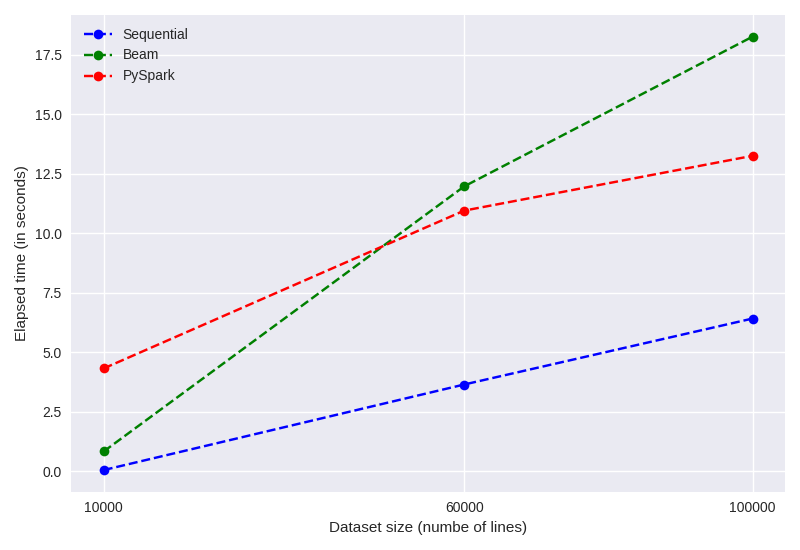
\includegraphics[width=.85\textwidth]{img/plot.png}
    \caption{Comparative analysis}
    \label{fig:plot}
\end{figure}

\vspace{\baselineskip}

As we can see in \Cref{fig:plot}, a sequential approach performed better than using Apache Beam or 
PySpark. This happens because the data sets considered are not large enough to overcome the 
overhead and latency introduced by using either Spark or Beam. However, for larger data sets, these 
are expected to perform better than a sequential approach due to their emphasis on processing 
elements in parallel.

\end{document}
